\xchapter{Experimentos}{Opcional}

Valores encontrados nas medições.

\section{Como avaliei}

Foi medido o tempo de resposta do linux comum para servir de referência e depois foi medido com o patch de tempo real. Foram realizadas medições com vários mecanismos de interrupção. Testes com cargas diferentes na CPU.

\subsection{Divisão por tipo de kernel}

\begin{itemize}
\item Normal
\item Preempt-RT
\item Xenomai
\end{itemize}

\subsection{Divisão por irqs}

\begin{itemize}
\item Softirq
\item Tasklet
\item Workqueue
\end{itemize}

\subsection{Divisão por carga na cpu}

\begin{itemize}
\item Ociosa
\item Um processo
\item Sobrecarga (256 processos)
\end{itemize}

\section{Resultados}

Preempt-RT mais lento na médio, melhor pior caso, menos variação.

Na figura \ref{tableau} temos uma figura.

\section{Resultados obtidos}

A primeira letra representa o kernel testado: (r)aspberry padrão ou (p)reempt-RT.
A segunda letra é o tipo de interrupção testado: (s)oftirq, (t)asklet, (w)orkqueue.
O terceiro caracter é a carga na cpu: 0 thread, 1 thread, (m)any threads (256).

\begin{figure}[!htb]
    \centering
    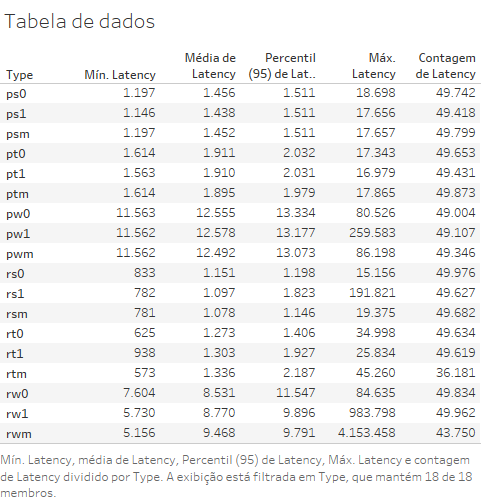
\includegraphics{graficos/tableau.png}
    \caption{Medições de latência}
    \label{tableau}
\end{figure}
